\documentclass[11pt]{article}

\usepackage{fontspec}
\usepackage{amsmath}
\usepackage{polyglossia}
\setmainlanguage{turkish}
\usepackage{geometry}
\geometry{a4paper, margin=2.3cm}
\usepackage{graphicx}
\usepackage{booktabs}
\usepackage{float}
\usepackage{xcolor}
\usepackage{hyperref}
\hypersetup{colorlinks=true, linkcolor=blue, urlcolor=blue}

\graphicspath{{figures/}}

\title{\textbf{YKS Cevap Anahtarı Atlası:\\
Sekiz Yıllık (2018--2025) Şık Dağılımı ve Yapı Analizi}}
\author{Hamza Yiğit Kültür \quad\textbullet\quad İsmail Güler\\[2pt]
\small \texttt{sallamasyon-yks} --- NVIDIA GH200 (Grace 72-core + H100)}
\date{\today}

\begin{document}
\maketitle

\begin{abstract}
\noindent
Bu rapor, önceki çalışmalardan farklı olarak \emph{hiçbir model veya tahmin
içermez}; tamamen \textbf{betimsel} bir ``atlas''tır. Amaç, YKS (TYT ve AYT)
sınavlarının cevap anahtarlarındaki genel yapıyı bol görselle resmetmektir.
Veri olarak \textbf{2018--2025 arası sekiz yılın tamamı} (toplam $2325$ geçerli
cevap, İPTAL hariç) kullanılır. \emph{Neden 2025 dahil?} Önceki raporlarda 2025
bir test seti olduğundan eğitime karıştırılmamıştı; ancak bu rapor öğrenme veya
tahmin yapmadığından sızıntı kavramı geçersizdir, dolayısıyla en eksiksiz
betimsel resmi vermek için 2025 de dahil edilmiştir. Bulgular özetle: şık
dağılımı düzgüne çok yakındır (en çok D $\%21.0$, en az E $\%19.0$; ki-kare
$=4.04$, anlamsız); ancak sınavların \emph{yapısında} belirgin örüntüler
vardır---her test içinde şıklar olağanüstü dengeli dağıtılır ve aynı şık ardarda
nadiren tekrarlanır ($\%13.2$).
\end{abstract}

\section{Veri Seti Künyesi}
Veri, ÖSYM'nin $16$ resmî sınav kitapçığından ($8$ yıl $\times$ TYT+AYT)
koordinat-tabanlı çıkarımla elde edilmiştir. Her test (ders) kendi içinde soru
sırasına göre tutulur. Tablo~\ref{tab:kunye} sınav yapısını gösterir.

\begin{table}[H]
\centering
\caption{Sınav yapısı: ders başına soru sayıları. AYT'de Sosyal Bilimler-2
testi, Din Kültürü almayanlar için Felsefe alternatifi nedeniyle $46$ cevap
içerir.}
\label{tab:kunye}
\begin{tabular}{lccccccc}
\toprule
Sınav & Türkçe & Sosyal & Mat. & Fen & Edeb.-Sos1 & Sos2 & Toplam \\
\midrule
TYT & 40 & 25 & 40 & 20 & --- & --- & 125 \\
AYT & --- & --- & 40 & 40 & 40 & 46 & 166

\\
\bottomrule
\end{tabular}
\end{table}
\noindent Sekiz yıl boyunca yalnızca \textbf{$3$ soru iptal} edilmiştir (hepsi
2019 TYT, 7.\ sorular); bunlar analiz dışı bırakılmıştır.

\section{Genel Şık Dağılımı}
Tablo~\ref{tab:overall} ve Şekil~\ref{fig:genel}, sekiz yılın birleşik şık
dağılımını verir. Dağılım düzgüne (her şık $\%20$) son derece yakındır:
en çok çıkan D ($\%21.0$) ile en az çıkan E ($\%19.0$) arasındaki fark yalnızca
$2$ puandır. Düzgün dağılıma karşı ki-kare testi $\chi^2=4.04$ olup $\%5$ kritik
değeri $9.49$'un altındadır; yani ``belirli bir şık daha sık çıkar'' iddiası
istatistiksel olarak \emph{desteklenmez}.

\begin{table}[H]
\centering
\caption{Genel şık dağılımı (\%), 2018--2025, $n=2325$.}
\label{tab:overall}
\begin{tabular}{lccccc}
\toprule
& A & B & C & D & E \\
\midrule
Genel (8 yıl) & 19.05 & 20.52 & 20.43 & 21.03 & 18.97

\\
\bottomrule
\end{tabular}
\end{table}

\begin{figure}[H]
\centering
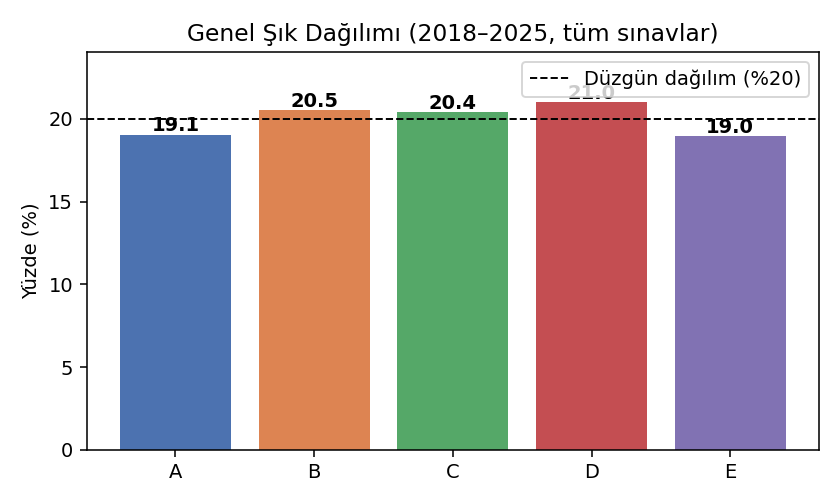
\includegraphics[width=0.62\textwidth]{atlas_genel.png}
\caption{Genel şık dağılımı. Her şık kendi sabit rengiyle gösterilir; siyah
kesikli çizgi düzgün dağılımı ($\%20$) işaretler.}
\label{fig:genel}
\end{figure}

\section{Zaman Boyutu: Yıllara Göre Yapı}
Şekil~\ref{fig:heatyil} ve Şekil~\ref{fig:trend}, dağılımın yıllar içindeki
seyrini gösterir. Genel resim \emph{kararlıdır}: hiçbir şık tutarlı bir
artış/azalış eğilimi göstermez; dalgalanmalar gürültü düzeyindedir. Örneğin E
şıkkı neredeyse her yıl en alttaki banttadır ($\%18$--$\%20$), ama hangi şıkkın
``en çok'' olduğu yıldan yıla değişir---bu da örüntünün öngörülemezliğini
pekiştirir.

\begin{figure}[H]
\centering
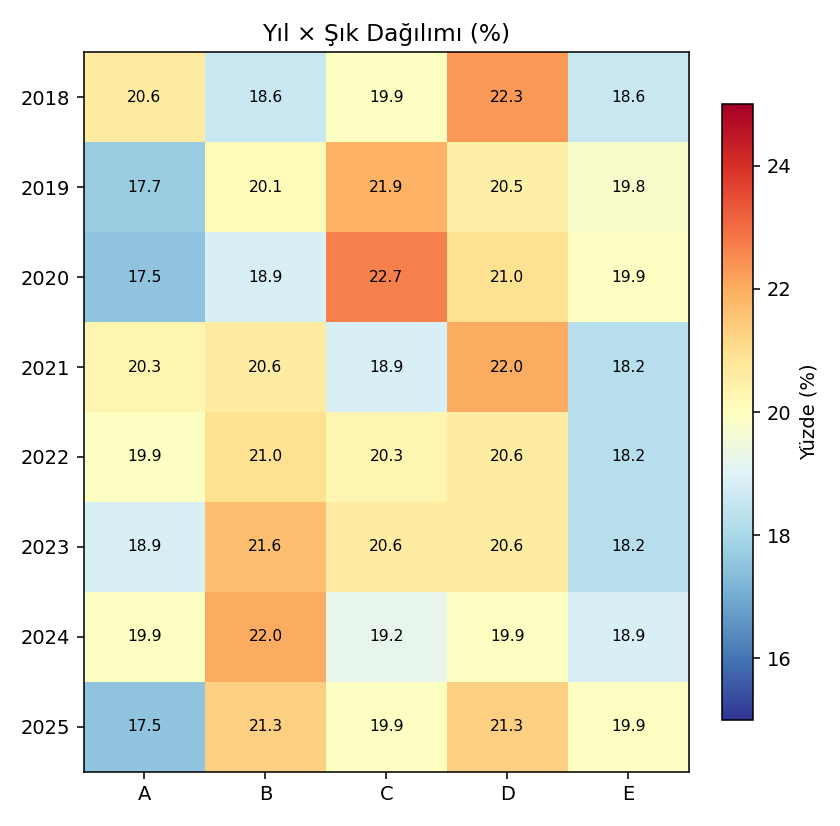
\includegraphics[width=0.6\textwidth]{atlas_heatmap_yil.png}
\caption{Yıl $\times$ şık ısı haritası. Her satır bir yılın ``şık parmak
izi''dir; renkler $\%15$--$\%25$ aralığında. Tüm hücreler $\%20$ civarında
kümelenir.}
\label{fig:heatyil}
\end{figure}

\begin{figure}[H]
\centering
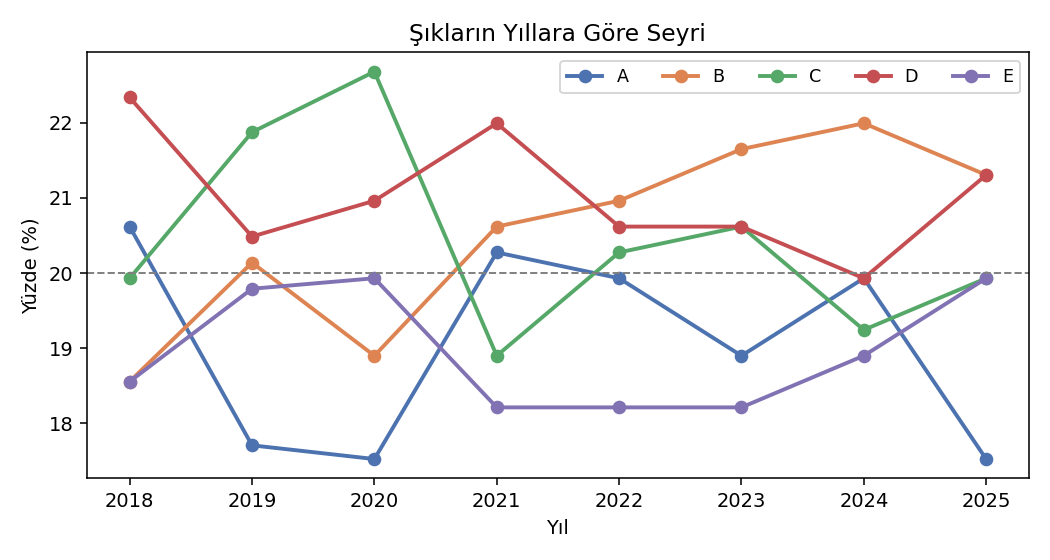
\includegraphics[width=0.78\textwidth]{atlas_yil_trend.png}
\caption{Şıkların yıllara göre yüzde seyri. Çizgiler $\%20$ etrafında
dalgalanır; belirgin bir trend yoktur.}
\label{fig:trend}
\end{figure}

\section{Ders Boyutu: Şık Parmak İzleri}
En ilginç betimsel yapı ders düzeyinde ortaya çıkar
(Tablo~\ref{tab:subject}, Şekil~\ref{fig:heatders}). Her dersin kendine özgü
bir ``şık parmak izi'' vardır: örneğin \textbf{Edebiyat-Sosyal1} dersinde C
belirgin biçimde öne çıkar ($\%22.8$) ve B düşüktür ($\%17.2$); buna karşın
Türkçe ve Fen'de D baskındır. Bu farklar mütevazıdır ama derslerin birbirinden
ayrıştığını gösterir.

\begin{table}[H]
\centering
\caption{Ders bazlı şık dağılımı (\%), 2018--2025.}
\label{tab:subject}
\begin{tabular}{lccccc}
\toprule
Ders & A & B & C & D & E \\
\midrule
Türkçe & 18.8 & 20.7 & 19.7 & 22.3 & 18.5 \\
Sosyal & 17.6 & 21.1 & 20.6 & 20.1 & 20.6 \\
Matematik & 18.3 & 22.1 & 20.7 & 21.0 & 18.0 \\
Fen & 19.0 & 19.8 & 19.6 & 21.7 & 20.0 \\
Edebiyat-Sosyal1 & 21.6 & 17.2 & 22.8 & 19.1 & 19.4 \\
Sosyal2 & 19.3 & 21.2 & 19.6 & 21.5 & 18.5

\\
\bottomrule
\end{tabular}
\end{table}

\begin{figure}[H]
\centering
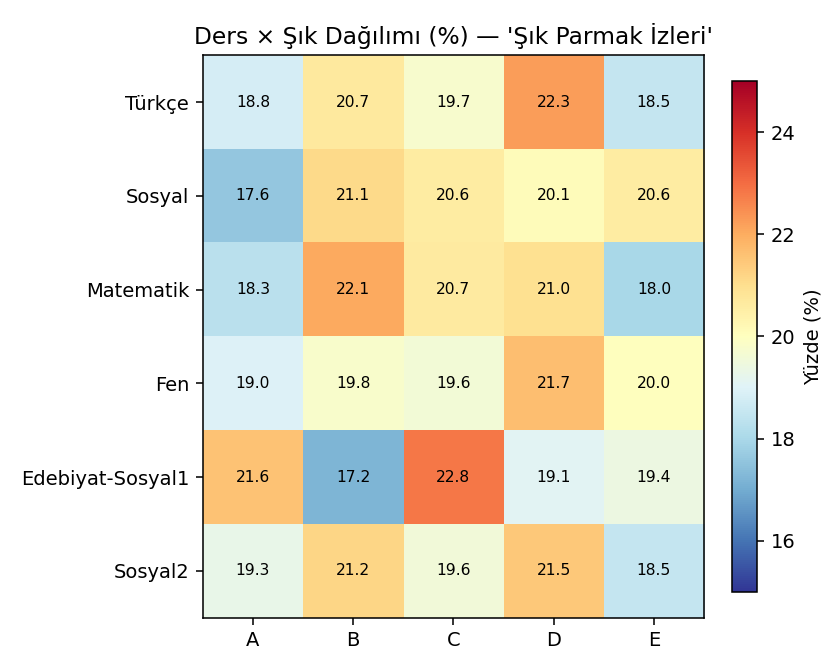
\includegraphics[width=0.72\textwidth]{atlas_heatmap_ders.png}
\caption{Ders $\times$ şık ısı haritası. Her satır o dersin şık dağılımı
vektörüdür. Edebiyat-Sosyal1'in C ağırlığı (kırmızı) açıkça görülür.}
\label{fig:heatders}
\end{figure}

\subsection{Şık Dağılımı ``Embedding'' Haritası}
Her ders ve her yıl, $5$ boyutlu bir şık-dağılımı vektörü olarak düşünülebilir.
Bu vektörleri temel bileşen analizi (PCA) ile iki boyuta indirgeyip
Şekil~\ref{fig:emb}'de gösteriyoruz: birbirine yakın noktalar, benzer şık
dağılımına sahip ders/yılları temsil eder. \textbf{Edebiyat-Sosyal1} sağ
tarafta belirgin bir aykırı (outlier) olarak ayrışır; yıllar ise merkezde
sıkı bir küme oluşturur (yıllar arası tutarlılığın görsel kanıtı).

\begin{figure}[H]
\centering
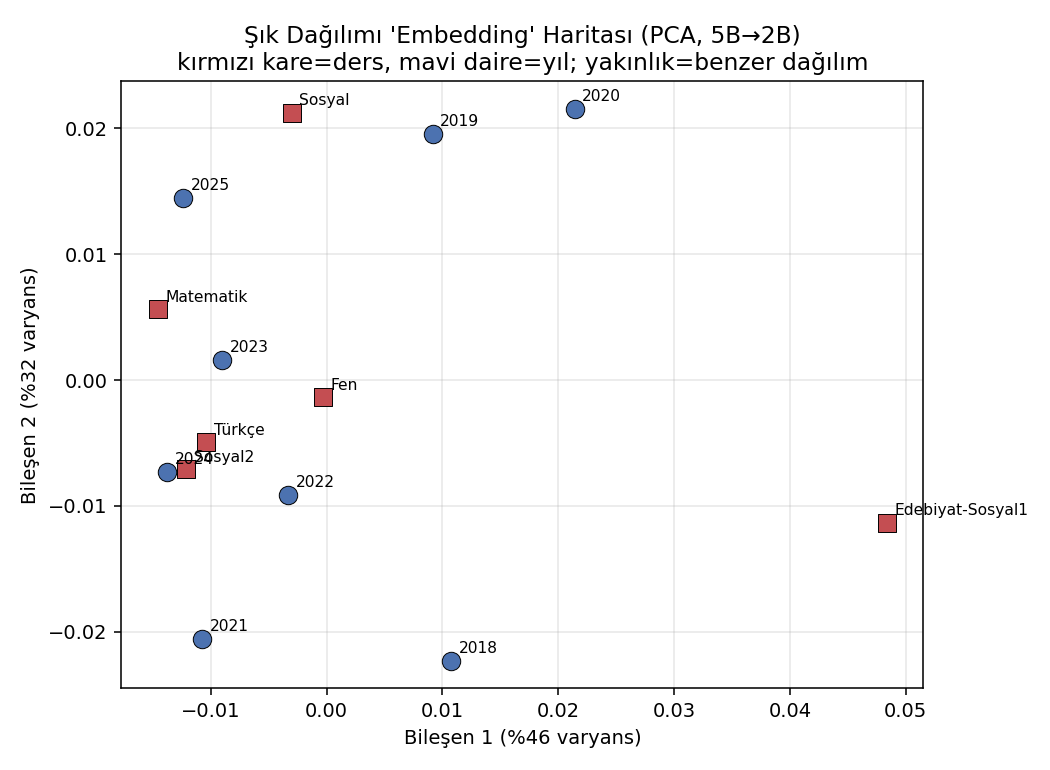
\includegraphics[width=0.78\textwidth]{atlas_embedding.png}
\caption{Şık dağılımı vektörlerinin PCA ile $2$B izdüşümü (kırmızı kare = ders,
mavi daire = yıl). Yakınlık, benzer şık dağılımı anlamına gelir.}
\label{fig:emb}
\end{figure}

\section{TYT ve AYT Karşılaştırması}
İki oturum birbirine çok benzer dağılıma sahiptir (Şekil~\ref{fig:tytayt});
en belirgin fark TYT'de A'nın ($\%18.2$), AYT'de E'nin ($\%18.4$) görece düşük
kalmasıdır. Pratik bir ayrım yoktur.

\begin{figure}[H]
\centering
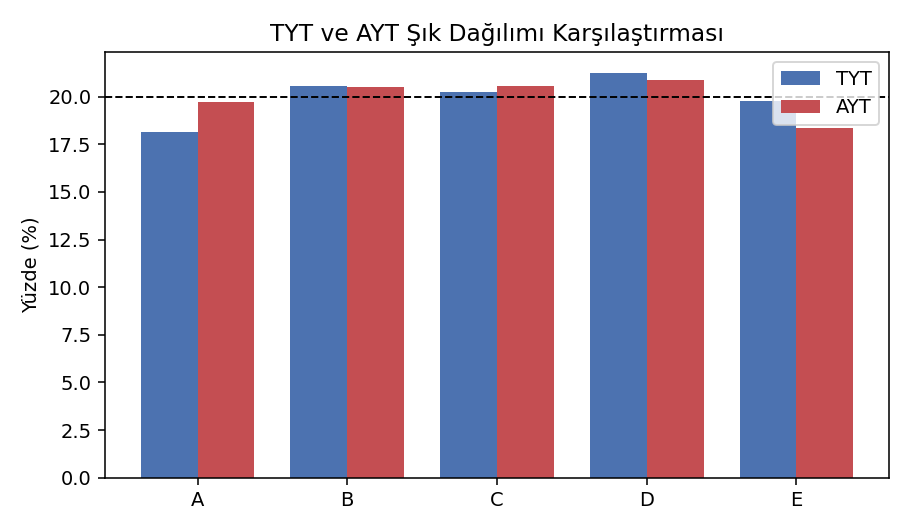
\includegraphics[width=0.62\textwidth]{atlas_tyt_ayt.png}
\caption{TYT ve AYT şık dağılımı karşılaştırması.}
\label{fig:tytayt}
\end{figure}

\section{Sıralı Yapı: Tekrar Kaçınması}
Dağılım düzgüne yakın olsa da, cevapların \emph{sırasında} güçlü bir örüntü
vardır. Şekil~\ref{fig:markov} ardışık geçiş matrisini gösterir: köşegen
(aynı şıkkın peş peşe gelmesi) tutarlı biçimde düşüktür (ortalama
$\%13.2$, rastgele $\%20$). Şekil~\ref{fig:gaprun} bunu iki açıdan
detaylandırır: (sol) aynı şık $2$--$3$ soru arayla bile beklenenden seyrek
görülür; (sağ) bir şık ne kadar üst üste gelmişse sonraki sorunun da aynı olma
olasılığı o kadar düşer---$2$ üst üsteden sonra $\%6$, $3$ üst üsteden sonra
$\%0$ (sekiz yılda hiç $4$'lü tekrar görülmemiştir).

\begin{figure}[H]
\centering
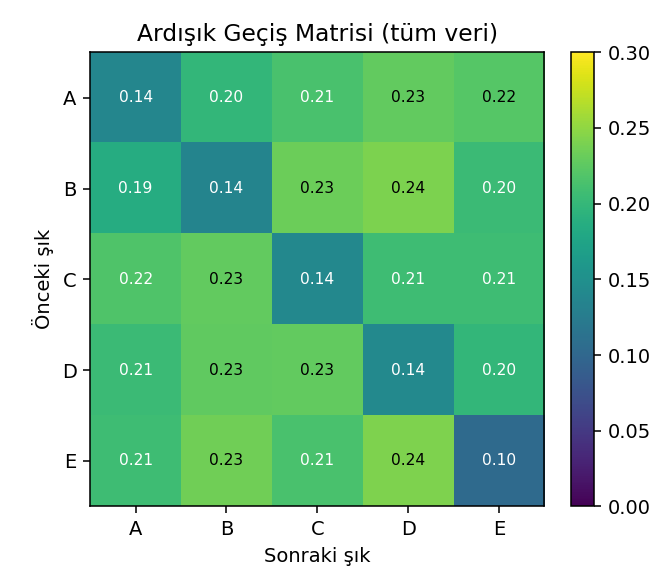
\includegraphics[width=0.5\textwidth]{atlas_markov.png}
\caption{Ardışık geçiş matrisi $P(\text{sonraki}\mid\text{önceki})$. Köşegenin
düşüklüğü, ardarda aynı şıkkın kaçınıldığını gösterir.}
\label{fig:markov}
\end{figure}

\begin{figure}[H]
\centering
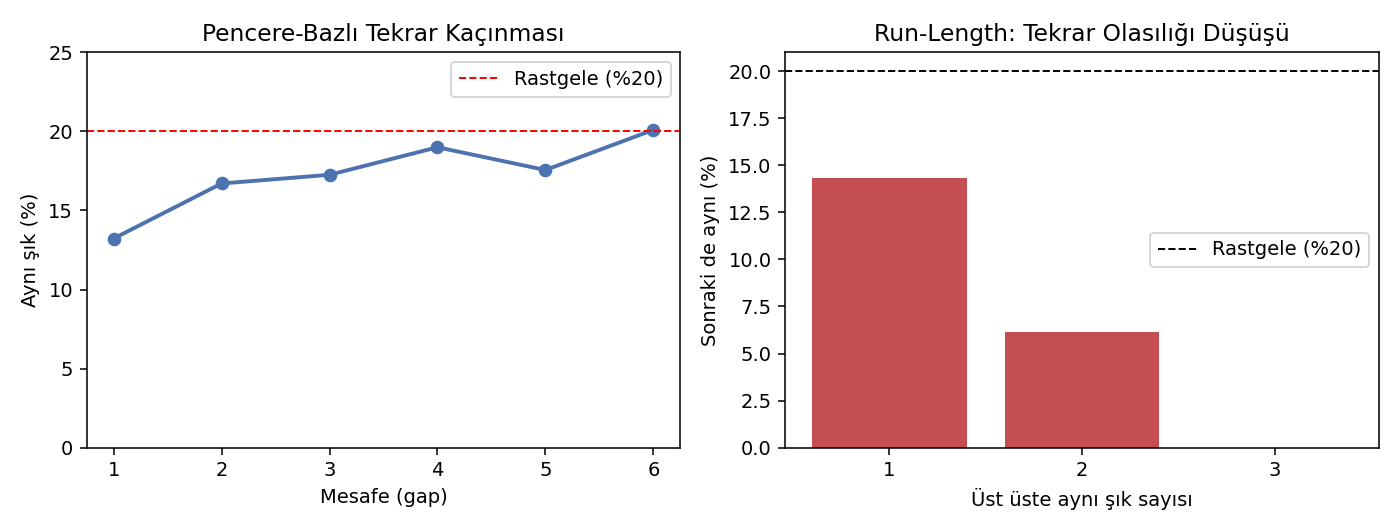
\includegraphics[width=0.95\textwidth]{atlas_gap_run.png}
\caption{Sol: mesafeye göre aynı-şık oranı. Sağ: üst üste tekrar sayısına göre
bir sonrakinin de aynı olma olasılığı.}
\label{fig:gaprun}
\end{figure}

\section{Denge Yapısı}
Sıralı kaçınmanın doğal sonucu, her testin \emph{içinde} şıkların olağanüstü
dengeli dağılmasıdır. Şekil~\ref{fig:denge}, her testteki şık sayılarının
standart sapmasını gösterir: gerçek sınavlar (ortalama $\sim 1.2$), aynı
uzunlukta rastgele dizilerin beklentisinin ($\sim 2.2$) çok altındadır. Yani
bir TYT testinde $40$ sorunun şıkları neredeyse $8$'er $8$'er dağıtılır.

\begin{figure}[H]
\centering
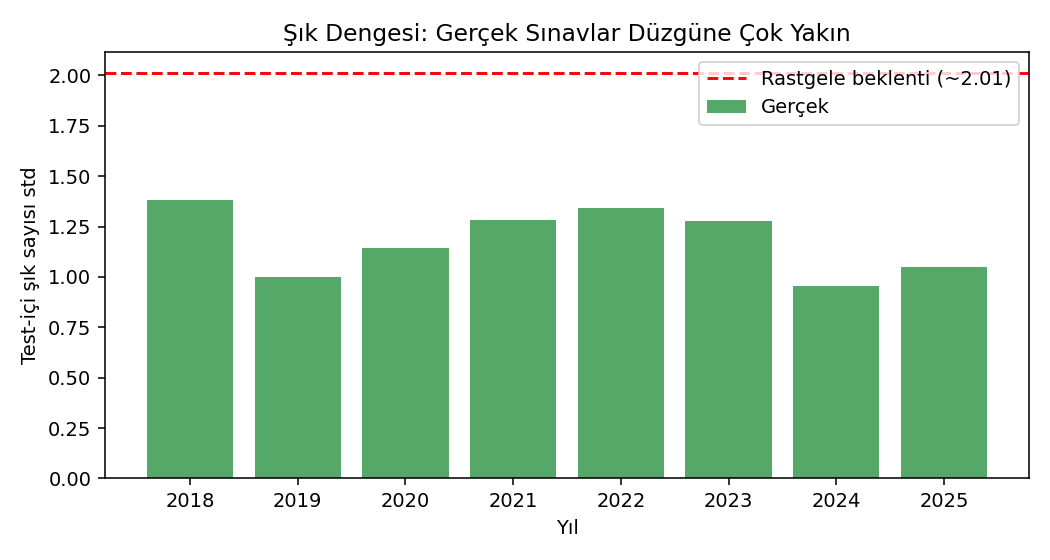
\includegraphics[width=0.78\textwidth]{atlas_denge.png}
\caption{Test-içi şık sayısı standart sapması (yıl bazlı). Gerçek değerler
rastgele beklentinin çok altındadır: şıklar dengeli dağıtılır.}
\label{fig:denge}
\end{figure}

\section{Özet Bulgular}
Sekiz yıllık atlasın damıtılmış çıkarımları:
\begin{itemize}
  \item \textbf{Dağılım düzgüne yakın.} En çok D ($\%21.0$), en az E ($\%19.0$);
  fark $2$ puan, ki-kare anlamsız. ``Hep bir şık'' stratejisi işe yaramaz.
  \item \textbf{Yıllar arası kararlı ama öngörülemez.} Genel resim sabit kalır;
  ancak hangi şıkkın o yıl ``en çok'' olacağı değişir.
  \item \textbf{Derslerin parmak izi var.} Özellikle Edebiyat-Sosyal1 (C
  ağırlıklı) diğerlerinden ayrışır; PCA haritası bunu görselleştirir.
  \item \textbf{TYT ve AYT neredeyse aynı.} Oturumlar arası anlamlı fark yok.
  \item \textbf{Güçlü sıralı yapı: tekrar kaçınması.} Ardarda aynı şık nadirdir
  ($\%13.2$), $4$'lü tekrar hiç yok; kaçınma $2$--$3$ soruluk pencereye yayılır.
  \item \textbf{Olağanüstü iç denge.} Her test içinde şıklar düzgüne çok yakın
  dağıtılır (std $\sim 1.2$ vs rastgele $\sim 2.2$).
\end{itemize}
Bu yapısal özellikler, önceki raporlarda ``sallamasyon'' için kullanılan
sinyallerin (dengeleme, tekrar kaçınması) \emph{betimsel temelini} oluşturur.

\paragraph{Tekrarlanabilirlik.} İşlem hattı: \texttt{extract\_answers.py}
$\rightarrow$ \texttt{analyze\_atlas.py} $\rightarrow$ \texttt{build\_report4.py}.

\end{document}
